\chapter*[GERENCIAMENTO DE PROJETO DE SOFTWARE]{GERENCIAMENTO DE PROJETO DE SOFTWARE}
\addcontentsline{toc}{chapter}{GERENCIAMENTO DE PROJETO DE SOFTWARE}
Gerenciar um projeto é aplicar conhecimentos, habilidades, ferramentas e técnicas às atividades do projeto a fim de atender aos requisitos de negócio. O gerenciamento inclui: identificar requisitos; adaptação às diferentes necessidades à medida que o projeto é planejado e realizado; balancear as restrições conflitantes do projeto que incluem, mas não se limitam a: escopo, qualidade, tempo, custo. \cite{ansi1998}

O empreendimento de um esforço temporário para criar um produto, serviço ou resultado exclusivo é denominado de projeto e possui um fluxo de atividades com início, meio e fim, cujo resultado é único. \cite{pmbok}

A crescente aceitação do gerenciamento de projetos indica que a aplicação desses elementos adequadamente pode ter um impacto significativo no sucesso de um projeto. \cite{pmbok}

A área de gerenciamento de projetos é uma das áreas que mais cresce em utilização no mundo, sendo, hoje, objetivo de investimento em capacitação e metodologia pela maioria das empresas. Em todo projeto, é senso comum que uma das principais dificuldades está na medição e na avaliação dos resultados obtidos, sejam eles resultados finais ou durante sua execução, relacionados a prazos, custos, qualidade, escopo, risco e outros. \cite{vargas2011} \citeonline{vargas2009}, elucida que a proposta do gerenciamento de projetos é estabelecer um processo estruturado e lógico para lidar com eventos que se caracterizam pela novidade, complexidade e dinâmica ambiental. Um dos fatores que impulsionam o gerenciamento de projetos é o crescimento da competitividade: quem for mais rápido e competente certamente conseguirá os melhores resultados. Essa competividade incita as empresas a conseguirem resultados com menos recursos, em um menor tempo e com mais qualidade.

Perguntas tais como: 1) Quanto tempo levará para desenvolver o software?; 2) Quanto custará o desenvolvimento do software?; dentre outras, são algumas das perguntas as quais todo patrocinador quer saber, pois antes de comprometer os recursos destinados a um projeto, o patrocinador deseja ter uma estimativa de prazo e custo. \cite{pfleeger2004}

Para se aplicar os conceitos de controle de processo faz-se necessário diferenciar duas modalidades, não concomitantes, aplicáveis ao gerenciamento de projetos: metodologia com processo definidos (ou prescritivos) e a metodologia empírica. De acordo com \cite{martins2007}, a primeira define o contexto do projeto e o escopo das entradas logo no início do projeto, enquanto que a outra define as entregas de forma abrangente e superficial, começando por um contexto inicial, que evolui e se adapta ao longo da execução e tem três pilares: transparência – os aspectos do processo que afetam o resultado final devem ser conhecidos e estarem visíveis para aqueles que controlam o processo; inspeção – vários aspectos do processo devem ser inspecionados para a detecção de variações; adaptação – surge com frequência mudanças no processo e nos recursos do processo que devem ser ajustado para minimizar maiores desvios. \cite{kenvolaro}

\section{GERENCIAMENTO TRADICIONAL}
A metodologia com processos definidos e prescritivos, também chamada de abordagem tradicional, é a mais adequada em situações onde os passos a serem executados, em geral, são conhecidos, como por exemplo, na implantação de uma infraestrutura de TI. Em projetos tradicionais, certo conjunto de entradas produzirá um conjunto específico de saídas. \cite{martins2007}

\subsection{O guia PMBOK}
O Guia PMBOK® fornece diretrizes para o gerenciamento de projetos individuais, define o gerenciamento e os conceitos relacionados, e descreve o ciclo de vida do gerenciamento de projetos e os processos relacionados. Tem por objetivo ser um guia com um conjunto de conhecimentos e boas práticas de aplicação. Não é uma metodologia, é uma referência básica, logo, a norma não é abrangente nem completa, possibilita o uso de ferramentas e metodologias distintas para implementar sua estrutura, e fornece um vocabulário comum para se discutir, escrever e aplicar o gerenciamento de projetos entre os membros envolvidos.

O guia é baseado em várias áreas e processos que organizam o trabalho a ser realizado durante o projeto. Os processos se relacionam e interagem segundo uma lógica definida para a condução do trabalho, realizada através de entradas, ferramentas e técnicas, e saídas.

\subsubsection{Ciclo de vida e a organização do projeto}
Consiste nas fases que oferecem uma estrutura básica para o gerenciamento do projeto, independente do trabalho especifico envolvido, todos os projetos podem ser mapeados para a estrutura do ciclo de vida: 1) Início do projeto; 2) Organização e preparação; 3) Execução do trabalho do projeto; e 4) Encerramento do projeto.  Esta estrutura pode ser visualizada na Figura \ref{fig1}. \cite{pmbok}
\begin{figure}[!htb]
	\centering
		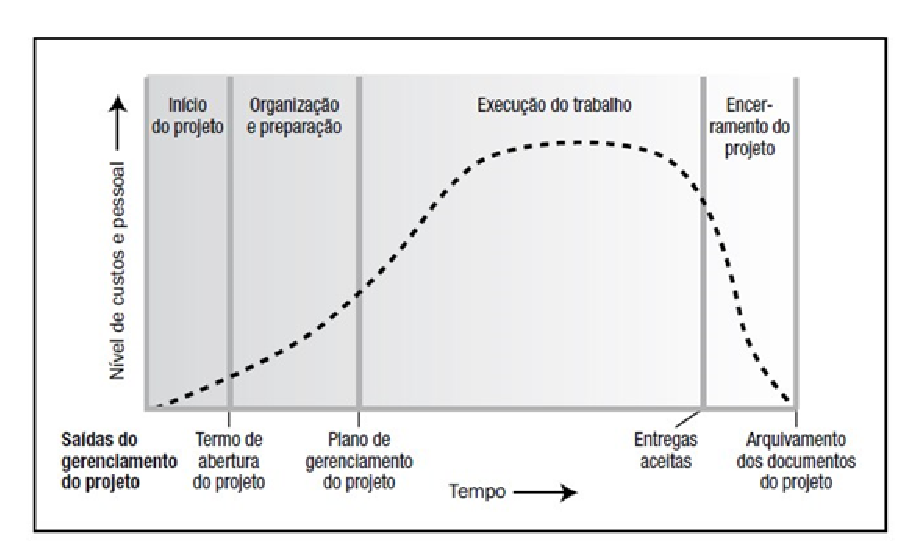
\includegraphics{figuras/fig1.eps}
		\caption{Nível típico de custos e pessoal ao longo do seu ciclo de vida. Fonte \cite{pmbok}}
		\label{fig1}
\end{figure}
\subsection{Grupos de Processos ou Fases}
Um processo é um conjunto de ações e atividades inter-relacionadas, que são executadas para alcançar um produto, resultado ou serviço predefinido. Os processos de gerenciamento de projetos são agrupados em cinco categorias:
\begin{itemize}
	\item Iniciação: Processos realizados para definir um novo projeto ou uma nova fase de um projeto existente através da obtenção de autorização para iniciar o projeto ou a fase. Nos processos de iniciação, o escopo inicial é definido e os recursos financeiros iniciais são comprometidos;
	\item Planejamento: Processos realizados para definir o escopo do projeto, refinar os objetivos e desenvolver o curso de ação necessário para alcançar os objetivos para os quais o projeto foi criado. Os processos de planejamento desenvolvem o plano de gerenciamento e os documentos do projeto que serão usados para executá-lo. Composto pelas atividades: Desenvolver o plano de gerenciamento do projeto; Coletar os requisitos; Estimar os recursos das atividades; Estimar as durações das atividades; Estimar os custos;Planejar a qualidade; Planejar o gerenciamento de riscos;
	\item Execução: Processos realizados para executar o trabalho definido no plano de gerenciamento do projeto para satisfazer as especificações do mesmo;
	\item Monitoramento e Controle: Processos necessários para acompanhar, revisar e regular o progresso e o desempenho do projeto, identificar todas as áreas nas quais serão necessárias mudanças no plano e iniciar as mudanças correspondentes. O principal benefício deste grupo de processos é que o desempenho do projeto é observado e mensurado de forma periódica e uniforme para identificar variações em relação ao plano de gerenciamento do mesmo. Inclui também 1) Controlar as mudanças e recomendar ações preventivas em antecipação a possíveis problemas; 2) Monitorar as atividades do projeto em relação ao plano de gerenciamento e à linha de base de desempenho do mesmo; e, 3) Influenciar os fatores que poderiam impedir o controle integrado de mudanças, para que somente as mudanças aprovadas sejam implementadas;
	\item Encerramento: Os processos executados para finalizar todas as atividades de todos os grupos de processos, visando encerrar formalmente o projeto ou a fase.
\end{itemize}

Os processos de gerenciamento de projetos são apresentados como elementos distintos com interfaces bem definidas. Porém, na prática eles se sobrepõem e sua aplicação é iterativa e muitos deles são repetidos durante o projeto. A natureza integrativa do gerenciamento de projetos requer que o grupo de processos de monitoramento e controle interaja com os outros grupos de processos, o de iniciação começa o projeto e o de encerramento termina, e o de planejamento fornece ao grupo de processos de execução o plano de gerenciamento e os documentos do projeto à medida que o projeto avança, conforme mostra a Figura \ref{grupoprocessospmi}
\begin{figure}[!htb]
	\centering
		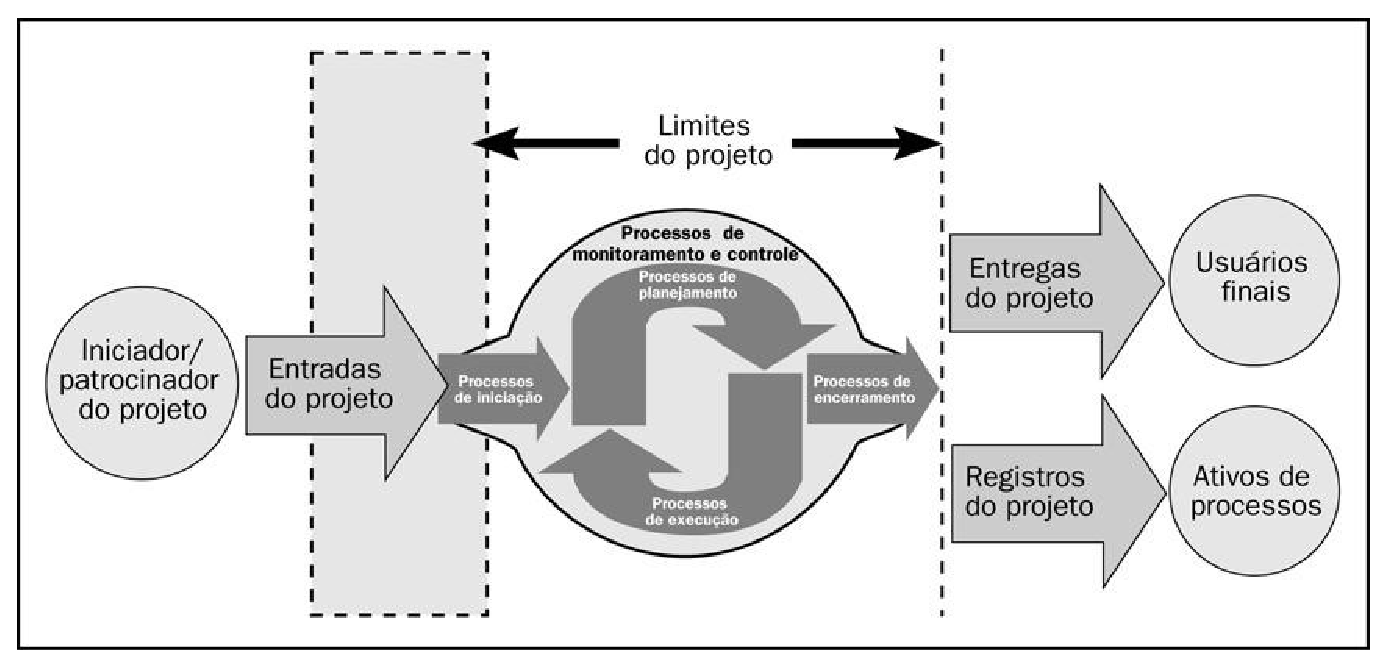
\includegraphics[scale=0.7]{figuras/grupoprocessospmi.eps}
		\caption{Grupo de Processos de Gerenciamento de Projetos Fonte \cite{pmbok}}
		\label{grupoprocessospmi}
\end{figure}
\subsubsection{Áreas de Conhecimento do PMBOK}
As áreas de conhecimento na prática são interativas e podem se sobrepor e interagir. As nove áreas são mostradas na Figura \ref{areasm}.
\begin{figure}[!htb]
	\centering
		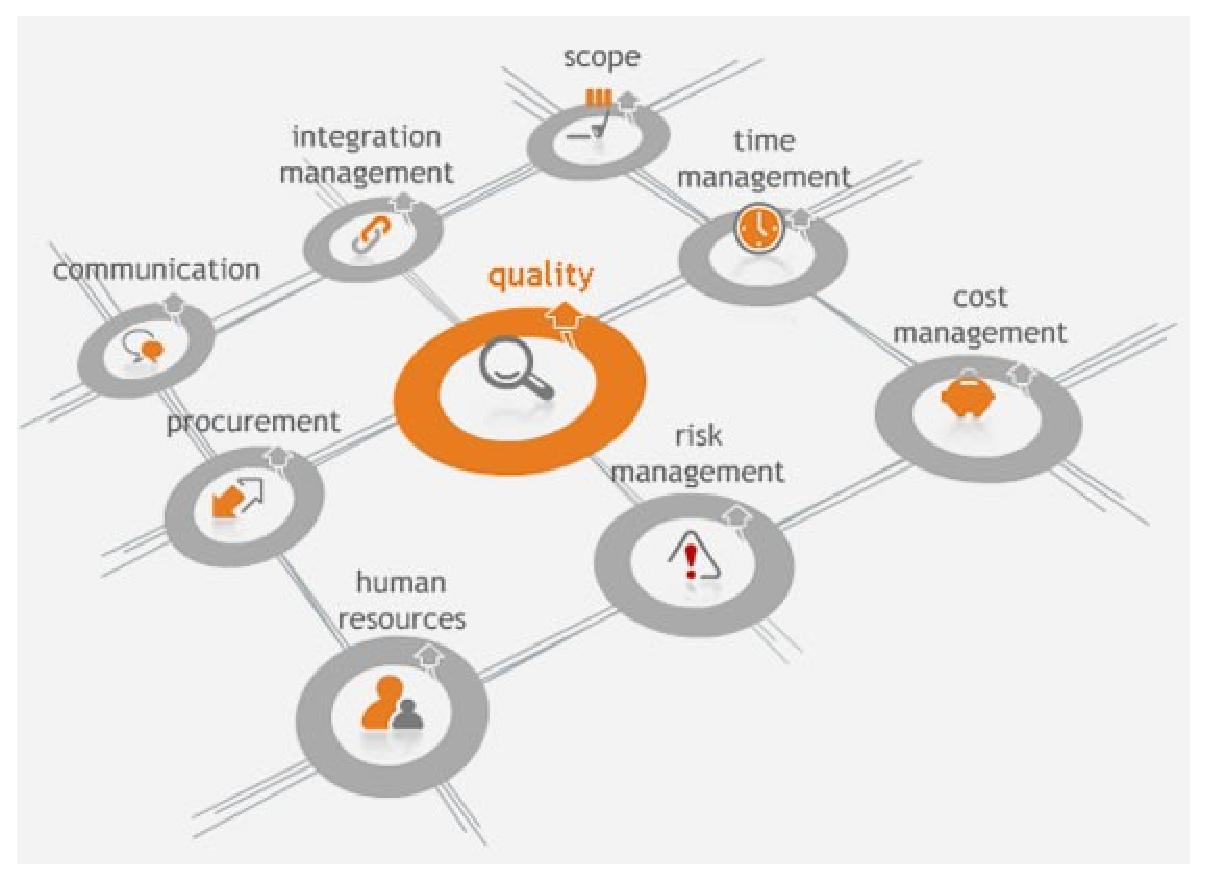
\includegraphics[scale=0.7]{figuras/areaspmi.eps}
		\caption{Áreas de Conhecimento PMB Fonte {http://www.allaboutxpert.com/nine-pmbok-areas}}
		\label{areaspmi}
\end{figure}

Gerenciamento das Aquisições: Inclui os processos necessários para comprar ou adquirir produtos, serviços ou resultados externos à equipe do projeto. \cite{pmbok}

Gerenciamento das Comunicações: Inclui os processos necessários para assegurar que as informações do projeto sejam geradas, coletadas, distribuídas, armazenadas, recuperadas e organizadas de maneira oportuna e apropriada. \cite{pmbok}

Gerenciamento dos Custos: Inclui os processos envolvidos em estimativas, orçamentos e controle dos custos, de modo que o projeto possa ser terminado dentro do orçamento aprovado. \cite{pmbok}

Gerenciamento do Escopo: Inclui os processos necessários para assegurar que o projeto inclui todo o trabalho necessário, e apenas o necessário, para terminar o projeto com sucesso. \cite{pmbok}

Gerenciamento da Integração: Inclui os processos e as atividades necessárias para identificar, definir, combinar, unificar e coordenar os vários processos e atividades dos grupos de processos de gerenciamento. \cite{pmbok}

Gerenciamento da Qualidade do projeto: Inclui os processos e as atividades da organização executora que determinam as políticas de qualidade, os objetivos e as responsabilidades, de modo que o projeto satisfaça às necessidades para as quais foi empreendido. \cite{pmbok}

Gerenciamento dos Recursos Humanos: Inclui os processos que organizam e gerenciam a equipe do projeto. \cite{pmbok}

Gerenciamento dos Riscos: Inclui os processos de planejamento, identificação, análise, planejamento de respostas, monitoramento e controle de riscos de um projeto. \cite{pmbok}

Gerenciamento do Tempo: Inclui os processos necessários para gerenciar o término pontual do projeto. \cite{pmbok}

\section{GERENCIAMENTO ÁGIL}

Muitas empresas de desenvolvimento de software estão se esforçando para se tornar mais ágeis. Equipes ágeis bem sucedidas estão produzindo software de alta qualidade para melhor atender, mais rapidamente, as necessidades dos usuários e com um custo menor do que as equipes tradicionais. \cite{cohn2010}

As empresas que tem tido sucesso na adoção de métodos ágeis, adotando um processo como o SCRUM combinado com outros métodos ágeis, estão evidenciando ganhos significativos de produtividade com diminuição de custos correspondentes. Elas são capazes de levar produtos ao mercado mais rapidamente e com um maior grau de satisfação do cliente, obtendo uma maior visibilidade para o processo de desenvolvimento, levando a uma maior previsibilidade, como consequência, e não como causa. E para estas empresas os termos “fora de controle”, “projetos que jamais serão concluídos” tornaram-se coisa do passado. \cite{cohn2010}

Um processo empírico requer frequentemente transparência, inspeções e adaptações durante o projeto, que é definido de forma inexata e pode gerar resultados imprevisíveis. É mais adequado e indicado para projetos de inovação e criação de novos produtos, como o desenvolvimento de software, por exemplo. A metodologia empírica, um dos pilares do SCRUM, é indicada nas situações onde as entradas do processo variam e processo é muito complexo para produzir resultados semelhantes. \cite{martins2007}

\subsection{SCRUM}
SCRUM é um conjunto de princípios e práticas que auxiliam equipes a entregar produtos em ciclos curtos, favorecendo um feedback rápido, melhoria continua e rápida adaptação à mudanças. Como guia do método de gerenciamento ágil, o SCRUM tem sido predominantemente usado para desenvolvimento de software, mas também está provando ser eficaz em esforços muito além funcionando muito bem para qualquer escopo complexo e inovador de trabalho. \cite{scrumalliance}

O SCRUM se baseia na ideia de controle de processo empírico, isto é, utiliza o conceito de progresso por meio da capacidade produtiva do time, e não de predição, para planejar e agendar entregas. SCRUM é um framework que, ao invés de fornecer completas e detalhadas descrições de como tudo deverá ser feito no projeto, permite ao time decidir por si só como deverá ser feito o trabalho, possibilitando saber qual a melhor forma de como resolver o problema apresentado. \cite{scrummethodology}

O SCRUM tem como alicerce a auto-organização e a multifuncionalidade da equipe: auto-organização, ou seja, a equipe é auto organizável, onde não há um líder geral que decide qual tarefa cada pessoa irá fazer, pois essas questões são decididas em equipe; multifuncionalidade, ou seja, cada membro da equipe precisa ter habilidade para pegar uma funcionalidade desde a ideia à implementação. \cite{mountaingoat}
O modelo de equipe no SCRUM é projetado para aperfeiçoar a flexibilidade, criatividade e produtividade. \cite{scrumguide}

O SCRUM consiste em Equipes associadas a seus papéis, eventos, artefatos e regras. E suporta todas as suas práticas em uma estrutura de modelo de ciclo de vida iterativo e incremental, como é mostrado na Figura \ref{esqueletoscrum}. \cite{scrumguide}

\begin{figure}[!htb]
	\centering
		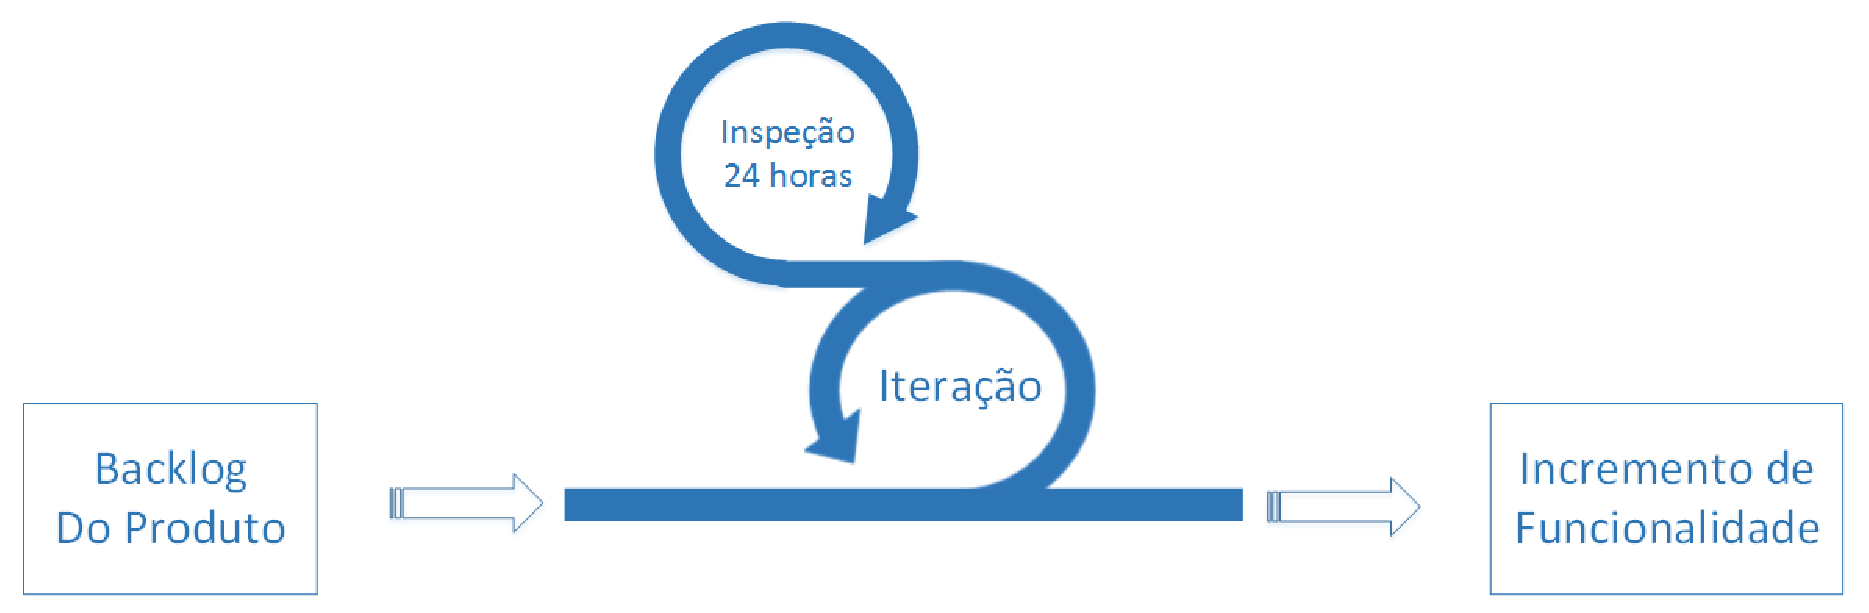
\includegraphics[scale=0.5]{figuras/esqueletoscrum.eps}
		\caption{Esqueleto SCRUM. Fonte \cite{schwaber2004}}
		\label{esqueletoscrum}
\end{figure}

Este esqueleto opera assim: no início de cada iteração, o time revisa o que deve ser feito. Depois selecionam o que acreditam que pode se tornar um incremento potencialmente entregável de uma funcionalidade no fim da iteração. O time é então deixado sozinho para fazer o melhor até o fim da iteração. No fim da iteração, o time apresenta para os \textit{stakeholders} o incremento da funcionalidade que foi construída para que seja inspecionando, aceito e também realizar mudanças no projeto. \cite{kenvolaro}

O coração do SCRUM ocorre durante a iteração. O time observa os requisitos, a tecnologia, e avalia as habilidades e capacidades de cada um. Em seguida, o time, coletivamente, debatem o melhor caminho conhecido para construir a funcionalidade, modificando dia a dia a abordagem assim que encontra novas complexidades, dificuldades ou surpresas, através das reuniões diárias. O time então discute o que falta ser feito e determina o melhor caminho para isso. \cite{schwaber2004}

\subsubsection{Papéis SCRUM}
Product Owner (PO)

O Product Owner é responsável por representar os interesses de todo mundo que possua uma participação ou interesse, no projeto e no sistema resultante, ou seja, representa o negócio, clientes ou usuários, e orienta a equipe a construir o produto certo. \cite{mountaingoat} Ele fornece a inicial e contínua base do projeto apresentando os requisitos gerais do projeto e os planos de entrega. O PO é o único responsável por gerenciar o Backlog do produto e deve garantir que a mais importante funcionalidade seja produzida primeiro. Isso é alcançado pela frequentemente priorização do Backlog do produto.\cite{schwaber2004}

Time de Desenvolvimento

O time consiste de membros que realizam o trabalho, são auto gerenciáveis, auto organizáveis, indivisíveis em sub-equipes, multifuncionais e possuem a responsabilidade de tornar o Backlog do produto em um incremento funcional de software em uma Sprint, além de gerenciar seus próprios trabalhos a serem feitos. O membros do time são responsáveis pelo sucesso de cada sprint e do projeto como um todo. \cite{schwaber2004}

SCRUMMaster (SM)

O SCRUMMaster é responsável por garantir o uso dos princípios e práticas do SCRUM. É muitas vezes considerado um treinador para a equipe, ajudando-a a fazer o melhor trabalho que puder, isso envolve a remoção de quaisquer impedimentos ao progresso, facilitando reuniões e interagindo diretamento com o Product Owner para garantir que o Backlog do produto esteja em “boa forma” e pronto para a próxima Sprint. \cite{schwaber2004}

\subsubsection{Fluxo}
A partir do documento de visão, o PO elabora, em alto nível, um plano de execução que inclua o Backlog do Produto(BP), que é uma lista de requisitos funcionais e não funcionais e prioriza o BP e o itens que estão no topo, que mais agregam valor, serão primeiramente implementados pela time. O BP é então dividido em releases e então as Sprints são planejadas.\cite{schwaber2004}

Cada Sprint inicia com a reunião de planejamento da Sprint, onde o PO e o time selecionam o que será feito na próxima Sprint. Essa reunião é dividida em duas partes, onde na primeira o time questiona o PO que deixa claro suas necessidades e o que deseja ao final da Sprint, e na segunda parte, o time planeja a Sprint e definem um conceito de incremento “pronto”. Os itens do BP selecionados para a sprint se tornam o Backlog da Sprint. Todos os dias o time se reúne por 15 minutos em uma reunião diária SCRUM, onde cada membro responde três perguntas:
\begin{itemize}
	\item O que eu fiz desde a reunião diária anterior? \cite{keith2010}
	\item O que eu farei até a próxima reunião diária? \cite{keith2010}
	\item O que me impede de desempenhar meu trabalho eficientemente? \cite{schwaber2004}
 \end{itemize} 

No fim da Sprint, realiza-se a reunião de revisão da Sprint, onde o time apresenta para o PO o que foi desenvolvido durante a Sprint. Os PO e stakeholders inspecionam o incremento e fazem adaptações no projeto para otimizar as chances de alcançar os objetivos. Antes de iniciar uma nova Sprint, o SCRUMMaster realiza uma reunião de retrospectiva, onde todos os membros do time participam, e baseado no SCRUM revisam todo o processo de desenvolvimento para torna-lo mais efetivo na próxima Sprint.\cite{schwaber2004}





